\documentclass[10pt,a4paper]{article}
\usepackage[T1]{fontenc}
\usepackage[utf8]{inputenc}
\usepackage{amsmath}
\usepackage{amsfonts}
\usepackage{amssymb}
\usepackage{tikz}
\usetikzlibrary{arrows.meta}

\begin{document}

\begin{center}
    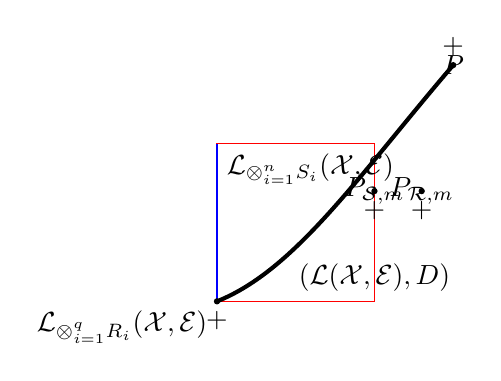
\begin{tikzpicture}[scale=2]
        % Define coordinates
        \coordinate (A) at (0,0);
        \coordinate (B) at (1,0);
        \coordinate (C) at (1,1);
        \coordinate (D) at (0,1);
        \coordinate (P) at (1.5, 1.5);
        \coordinate (PSm) at (1,0.7);
        \coordinate (PRm) at (1.3,0.7);
        
        % Draw the red box
        \draw[red] (A) -- (B) -- (C) -- (D) -- cycle;
        
        % Draw the blue line
        \draw[blue] (A) -- (D);
        
        % Draw the black line
        \draw[line width=1.5pt] (A) .. controls (0.5, 0.2) and (0.9, 0.8) .. (P);
        
        % Label points
        \node at (PSm) {$P_{\mathcal{S}, m}$};
        \node at (PRm) {$P_{\mathcal{R}, m}$};
        \node at (P) {$P$};
        \node at (A) [below left] {$\mathcal{L}_{\otimes_{i=1}^{q} R_i}(\mathcal{X}, \mathcal{E})$};
        \node at (D) [below right] {$\mathcal{L}_{\otimes_{i=1}^{n} S_i}(\mathcal{X}, \mathcal{E})$};
        \node at (B) [above] {$(\mathcal{L}(\mathcal{X}, \mathcal{E}), D)$};
        
        % Markers
        \fill (P) circle (0.02) node[anchor=south]{+};
        \fill (PSm) circle (0.02) node[anchor=north]{+};
        \fill (PRm) circle (0.02) node[anchor=north]{+};
        \fill (A) circle (0.02) node[anchor=north]{+};
    \end{tikzpicture}
\end{center}

Hierarchical decomposition of divergence in terms of orthogonal projections with respect to a partition \(\mathcal{R}\) and its refinement \(\mathcal{S}\).

\end{document}